\section{业界智能客服系统现状}
\zihao{-4}
\label{section:peer-system}

本文基于在线呼叫中心面向客服领域,选择了当前具有代表性的三家(款)呼叫中心智能客服系统,
阿里“ALIME”、京东“JIMI”和网易“七鱼”进行分析、对比和评价。
由于包括这三家在内的业内主要智能客服问答系统均为开源,因此本文根据其网站介绍、演示Demo和使用说明
对其工作原理和实现方式进行合理推测,并建立一套评价标准,对其进行对比和评价。

\subsection{ALIME}
\label{subsection:alime}
阿里“ALIME”是阿里巴巴推出的在线呼叫中心客服对话机器人平台,其核心场景为:
在商家促销活动时(如“年中6·18”、“双11”等)人工客服资源紧张,无法顾及到所有顾客,
此时,若顾客无法及时得到关于商品信息的应答,则销售机会转瞬即逝,给商家带来损失;
在平常时段,大型商家具有固定的工作时间,往往面临夜间无人或缺人值班的情况,
而小商家则一般身兼数职,分身乏术。因此阿里针对此类场景提出了检索式“ALIME”客服对话机器人平台。

“ALIME”平台系统由“千牛店小蜜”和“阿里小蜜”两部分组成,完整商业版于2017年6月正式上线。
其中“千牛店小蜜”面向淘宝商家,支持所有淘宝和天猫店铺,是阿里商家版智能客服机器人;
“阿里小蜜”面向淘宝顾客,支持所有淘宝顾客,是阿里顾客版智能客服机器人。

“ALIME-千牛店小蜜”(以下简称“店小蜜”)目前主要的功能有:
识别顾客购物意图、判断顾客购物缺失信息、查询顾客购物信息和一定时限内上下文识别等。
具体产品功能和知识库见表\ref{table:alime-ability}和表\ref{table:alime-kd}\wordnote{
    其中,“—”表示无,“...”表示省略。
}
。
\begin{table*}[h]

\parbox[t]{0.5\textwidth}{
\centering
\caption{\label{table:alime-ability} “ALIME-千牛店小蜜”产品能力}

\begin{tabular}{ccc}
\toprule
售前服务  &   订单服务  &   售后服务\\
\midrule
回复询价    &   回复发货时间  &   回复退货流程\\
回复询单    &   确认发货快递  &   回复退货事项\\
关联商品回复  &   确认订单修改  &   —\\
解决包邮议价  &   —  &   —\\
回复商品优惠  &   —  &   —\\
回复活动内容  &   —  &   —\\
\bottomrule
\end{tabular}
}
\parbox[t]{0.5\textwidth}{
\centering
\caption{\label{table:alime-kd} “ALIME-千牛店小蜜”电商知识库}

\begin{tabular}{cc}
\toprule
通用知识点 &   行业知识点\\
\midrule
基础商品问题    &   手机行业\\
活动优惠问题    &   服务行业\\
下单付款问题    &   鞋类行业\\
商品物流问题    &   零食行业\\
售后退款问题    &   ...\\
店铺服务问题    &   ...\\
聊天互动问题    &   ...\\
\bottomrule
\end{tabular}
}

\end{table*}

本小节以图\ref{figure:alime_case}为例详细阐述“ALIME”对话过程。
图\ref{figure:alime_case}中展示了“ALIME”的两个对话案例。
其中,图\ref{figure:alime_case1}中为“店小蜜”在服装类淘宝商家“森马”中的应用,即“森小蜜”。
由图可知,顾客:“这件衣服身高160选多大码合适”\wordnote{
    结合后文,这里的“衣服”应该在之前对话中进行过明确。
},
“森小蜜”:“请问体重是多少公斤?”,
顾客:“50”,“森小蜜”:“身高160.0公分,体重50.0公斤,...,推荐[修身M,宽松L]码...”;
图\ref{figure:alime_case2}为“阿里小蜜”在顾客查询中的应用。
\begin{figure*}[ht]
    \centering
    \begin{minipage}{0.5\textwidth}
        \centering
        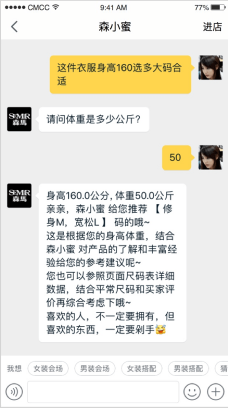
\includegraphics[width=0.6\textwidth]{alime_case1.png}
        \subcaption{\label{figure:alime_case1} “千牛店小蜜”案例}
    \end{minipage}%
    \begin{minipage}{0.5\textwidth}
        \centering
        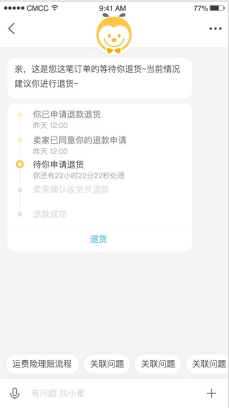
\includegraphics[width=0.6\textwidth]{alime_case2.png}
        \subcaption{\label{figure:alime_case2} “阿里小蜜”案例}
    \end{minipage}%
    \caption{\label{figure:alime_case} 阿里“ALIME”案例}
\end{figure*}

\textbullet{}问答系统首先接收到顾客的输入“这件衣服身高160选多大码合适”。

执行步骤\ding{172}:结合上下文根据语义分析模型对该语句进行分词和关键词抽取。

从该句中抽取关键词“衣服”、“身高”-“160”、“多大”、“码”。
其中,根据“多大”判定该语句为疑问句;
根据“衣服”和上文关联,确定该语句中“衣服”的目标;
根据“键-值”关系“身高-160”和“码”,确定“衣服”的部分商品信息。
综合上述抽取和分析过程,确定该顾客的意图,
即:连接该商家电商服装知识库,查询在“衣服”等于当前衣服、“身高”等于160时的码数,
完成识别购物意图功能。

执行步骤\ding{173}:执行顾客意图,进行检索操作。

此时,根据电商知识库的返回为“衣服”、“身高”、“体重”和“码数”的组合,返回值不唯一,
体现在“码数”和“体重”的返回数量上,因此判定缺失“体重”信息。

执行步骤\ding{174}:询问顾客购物缺失信息。

向顾客提问“体重”信息,以补全购物信息,以获取缺失查询条件“体重”。

\textbullet{}问答系统抛出应答“请问体重是多少公斤”。

\textbullet{}问答系统接受顾客输入“50”。

执行步骤\ding{172}:结合上下文根据语义分析模型对该语句进行分词和关键词抽取。

获取到体重信息“键-值”关系“\mbox{体重}:\mbox{公斤}-50”\wordnote{
    “键-值”关系$pair\{key-value\}$实际是$pair\{index-value\}$关系,即索引-值关系。
    因此键值有多种形式,如上文中身高信息的“键-值”关系为“身高-160”,
    此处体重信息的“键-值”关系为“\mbox{体重}:\mbox{公斤}-50”等。
}
,得到完整顾客信息查询条件。

执行步骤\ding{173}:执行顾客意图,进行检索操作。

此时,根据电商知识库的返回为“衣服”、“身高”、“体重”和“码数”的组合,返回值唯一,获得“码数”信息。

执行步骤\ding{175}:返回顾客购物缺失信息。

\textbullet{}问答系统抛出应答“身高160.0公分,体重50.0公斤,...,推荐[修身M,宽松L]码...”。

这里的问答系统应带内容中虽然带有“推荐”字样,
但实质将查询结果[修身M,宽松L]带入到应答模版“身高*公分,体重*公斤,...,推荐[*]码...”,
并非推荐系统的推荐结果。

\begin{figure*}[!htp]
    \centering
    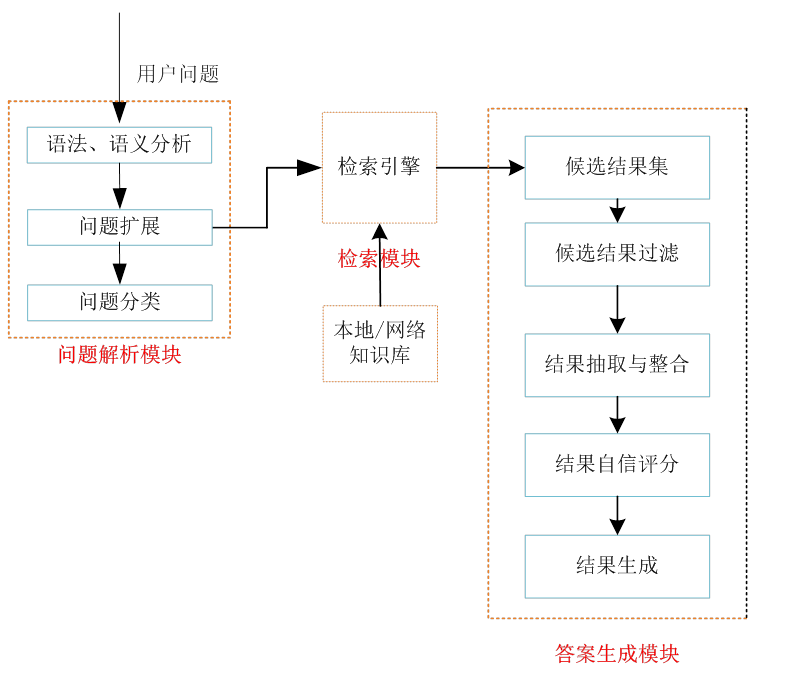
\includegraphics[width=0.8\textwidth]{QA_step.png}
    \caption{\label{figure:qa} 问答系统流程}
\end{figure*}

现阶段业界普遍采用的问答系统流程见图\ref{figure:qa}。

\subsection{JIMI}
\label{subsection:jimi}
京东“JIMI”(JD Instant Messaging intelligence)是京东推出的检索式智能客服机器人,
旨在为京东顾客提供更好的购物和咨询体验。
其应用场景与阿里“ALIME”相同,但比“ALIME”上线更早,于2013年3月通过测试上线,
具体过程见表\ref{table:jimi-event},功能见表\ref{table:jimi-ability}。
% \begin{table*}[h]

% \centering
% \caption{\label{table:jimi} “JIMI”主要上线事件}

% \begin{tabular}{cc}
% \toprule
% 日期  &   事件  \\
% \midrule
% 2013年3月1日    &   JIMI通过测试正式上线\\
% 2013年11月1日   &   JIMI登上促销活动页面\\
% 2013年8月7日    &   服装类商家店铺JIMI上线\\
% 2013年8月21日   &   3C全部单品页JIMI上线\\
% \bottomrule
% \end{tabular}

% \end{table*}
\begin{table*}[h]

\parbox[t]{0.5\textwidth}{
\centering
\caption{\label{table:jimi-event} “JIMI”主要上线事件}

\begin{tabular}{cc}
\toprule
日期  &   事件  \\
\midrule
2013年3月1日    &   JIMI通过测试正式上线\\
2013年11月1日   &   JIMI登上促销活动页面\\
2013年8月7日    &   服装类商家店铺JIMI上线\\
2013年8月21日   &   3C全部单品页JIMI上线\\
\bottomrule
\end{tabular}

}
\parbox[t]{0.5\textwidth}{
\centering
\caption{\label{table:jimi-ability} “JIMI”产品能力}

\begin{tabular}{ccc}
\toprule
售前服务 &  售后服务  &   闲聊服务\\
\midrule
查询订单    &  回复退换货流程  &   笑话\\
取消订单    &  回复退换货事项   &   对诗\\
回复商品优惠  &   —  &   天气查询\\
回复活动内容  &   —  &   —\\
\bottomrule
\end{tabular}
}

\end{table*}
\begin{table*}[!htp]

\centering
\caption{\label{table:jimi-skill} “JIMI”提问技巧}

\begin{tabular*}{\textwidth}{c>{\centering\arraybackslash}m{0.3\textwidth}>{\centering\arraybackslash}m{0.6\textwidth}}
\toprule
技巧  &   错误举例  &  描述\\
\midrule
省略问候语&“您好”、“请问一下”、“在吗”等&\makecell{不需要添加问候语\\直接陈述问题}\\
问题简洁&“我的订单不想要了,可以吗”&\makecell{只需问“我要取消订单”\\避免冗长}\\
提问完整&“怎么解决呢”&\makecell{“地址错了,怎么解决”或“地址错了,怎么办”\\避免一个问题两次发送}\\
单次提问&“您好,我京东的注册密码及支付密码忘记了,请问该怎么找回呢”&\makecell{“如何找回京东注册密码”、“\mbox{支付密码忘记},\mbox{怎么办}”\\避免一个问题包含两个提问}\\
减少错字&“优汇劵”、“那个商品有活动”&\makecell{“优惠卷”、“哪个商品有活动”\\避免错别字}\\
问题引导&-&\makecell{输入关键词后,系统会匹配一系列相关的问题\\可以直接点击相似或同类问题,直接获取答案}\\
\bottomrule
\end{tabular*}

\end{table*}
\begin{figure*}[!htp]
    \centering
    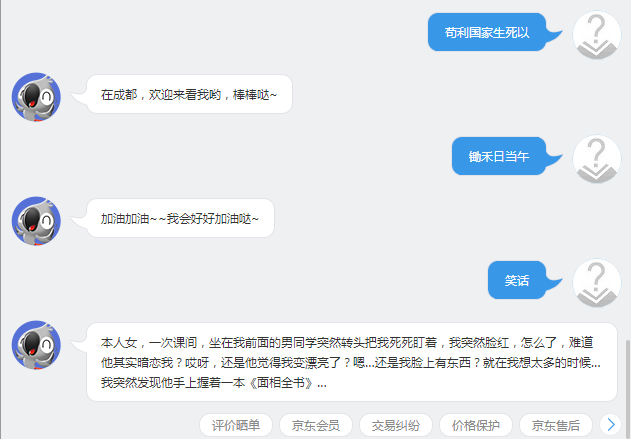
\includegraphics[width=0.8\textwidth]{jimi_chat1.png}
    \caption{\label{figure:jimi_chat} 京东“JIMI”案例}
\end{figure*}

“JIMI”和“ALIME”均为检索式智能客服机器人,
通过表\ref{table:jimi-skill}和图\ref{figure:jimi_chat}
可推测出“JIMI”的工作原理和实现方式与“ALIME”类似。
根据表\ref{table:jimi-skill}中“提问完整”技巧可知,
“JIMI”相比“ALIME”缺失了一定的上文关联能力,且对输入要求更加苛刻。

功能上,“JIMI”比“ALIME”多出了包括“笑话”、“对诗”和“天气查询”的闲聊服务功能。
首先“天气查询”本质上并不属于聊天的范畴而属于较为简单不涉及复杂语义分析的检索功能;
其次,通过实际测试,如图\ref{figure:jimi_chat}可知,“JIMI”所提供的“笑话”和“对诗”能力亦不属于生成式对话系统。
“前者”需要顾客输入关键词“笑话”,系统随后从笑话知识库中随机抽取一段笑话抛出;
“后者”甚至不能识别一些经典诗句,以致系统完全误解顾客意图。
因此“JIMI”的闲聊服务功能并不出彩,甚至给顾客造成了预期落差,产生了消极的对话体验。

虽然“JIMI”在对话窗体底部提供了“评价晒单”、“京东会员”、“交易纠纷”和“京东售后”等查询入口,
相比“ALIME”给顾客带来了一定程度的便利。
但这些入口严格意义上并不属于本文所研究的客服问答系统,因此不归为京东“JIMI”的优势功能。

\subsection{七鱼}
\label{subsection:qiyu}

网易“七鱼”是网易研发服务企业的检索式智能问答系统。其应用场景亦与“ALIME”和“JIMI”类似,
于2016年4月上线。
“七鱼”与“ALIME”、“JIMI”同为检索式问答系统。通过企业自建的知识库和相似词库完成关键词抽取和语义识别,
如图\ref{figure:wyqy_kd}所示。
\begin{figure*}[!htp]
    \centering
    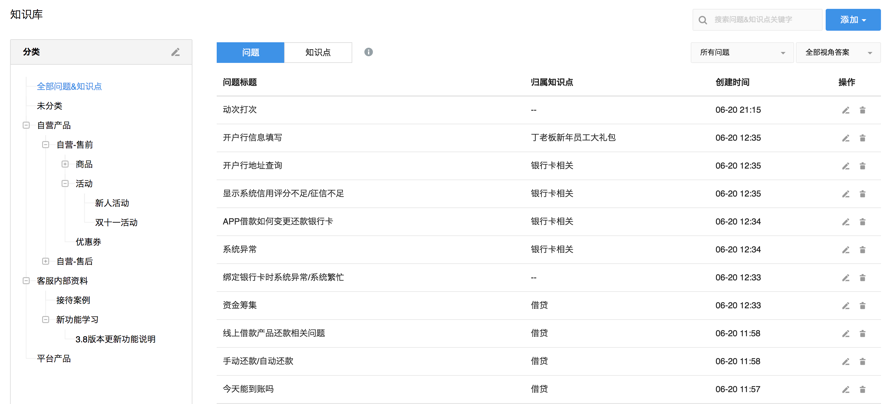
\includegraphics[width=\textwidth]{wyqy_kd.png}
    \caption{\label{figure:wyqy_kd} 网易“七鱼”知识库}
\end{figure*}

网易“七鱼”作为国内智能客服问答领域新生产品的代表,同样采取问题-知识检索的方式构建智能问答系统。
相较于“ALIME”、“JIMI”,“七鱼”采用开放网站、APP和微信接口的方式获取企业用户\wordnote{
    \url{https://github.com/qiyukf}
},
然而这种渠道优势如同“JIMI”查询入口亦不属于问答系统的原理范畴,因此同样不归为其优势功能。

\subsection{评价指标}
\label{subsection:evaluation}

目前由美国国家标准技术句主持的文本检索会议(TREC)
针对TREC/QA任务下的问答系统提出了一套评价指标\citep{voorhees2000building}。
该套评价指标针对不同类别问题略有不同,总体由3个部分组成,
实例查询准确率(Instance Precision)、实例查询召回率(Instance Recall)和F值(F1 Measures)。
其中,实例查询准确率指的是问答系统给出的正确答案占给出的全部答案的比例,
实例查询召回率指的是问答系统给出的正确答案的数量占所有正确答案的比例,F值则是实例查询准确率和实例查询召回率的调和平均值。
然而这套评价指标并不完全符合客服问答系统。

企业作为客服问答系统的使用者, 核心需求为保持和扩展顾客群体,进而提高盈利。
当然,反馈给顾客正确的应答毫无疑问为非常重要的问答系统评价指标,
然而在企业的需求下,在无法给予顾客准确应答的情况时,给予顾客以适当的情感抚慰,也有可能挽留顾客并满足顾客的情感需求。
顾客作为客服问答系统的参与主体,不局限于答案准确率,同时希望在快速获取准确答案的同时感受类人的交互。
因此应当考虑建立时间分数和智能客服类人程度的评价标准。

时间分数是客服回答机器人与顾客对话时间的分数。顾客和企业都希望能够以尽量短的时间得到(给出)正确的答案。
此处的时间可定义为对话时长或交互次数。对话时长目前主要受客户打字速度或其他因素的影响,若采用对话时长作为时间的评价标准,
则会产生相比交互次数更大的误差,因此以在顾客最终得到正确答案时客户回答机器人与顾客对话的交互次数作为时间分数的影响因素。
在顾客得到正确答案时,交互次数越少,时间分数越高,反之,交互次数越多,时间分数越低;在顾客无法得到正确答案时,时间分数为0。

知名的机器类人程度评价有“图灵测试”。
若在智能客服问答系统中建立图灵测试,
则需要取消问答系统中转接人工客服的功能并对顾客进行一定的误导以使顾客无法先验客服身份,
但此方法代价颇高。
由于自然语言的天然复杂性,现阶段的客服问答系统均无法达到较高的人类自然语言相似度。
机器无法理解自然语言表述导致无法抛出正确应答,顾客又无法转接人工客服,极易使顾客失去耐心和信任,造成顾客流失,
而这正是企业最不愿发生的。
因此图灵测试不适合直接应用与智能客服的类人评价。具体如何建立一套合理和有效的类人评价方法,值得学界和业界的继续探讨。

综上所述,本文借鉴TREC/QA评价体系,根据智能客服问答系统情景综合考虑了问答系统的应答质量、时间和类人程度因素,
提出了准确率、召回率、F值、时间分数和类人程度五元的综合评价体系。
其中,
准确率为问答系统给出的正确答案占给出的全部答案的比例;
召回率为问答系统给出的正确答案的数量占所有正确答案的比例;
F值为准确率和召回率的调和平均值;
时间分数为问答系统与顾客交互次数的函数;
类人程度是问答系统应答与人工客服应答的相似程度。

\subsection{系统对比}

由于缺乏相应训练集、测试集、知识库和完整评价指标,故此小节未完成...